\section{Aprofundamento}

\begin{frame}{Código fonte do computador}
	\begin{block}{}
		\begin{itemize}
			\item Codificação simples para entender dados e transformá-los em informação.
			\item Na “linguagem” de computador, temos apenas 0's e 1's.
			\item Em sua base, os computadores são capazes de distinguir \textbf{dois estados} distintos.
		\end{itemize}
	\end{block}

	\centering
	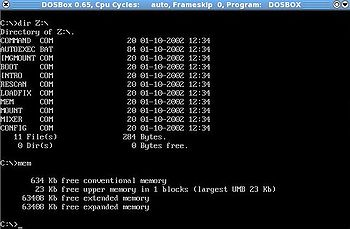
\includegraphics[width=0.6\linewidth]{Figuras/Ch02/fig1}
\end{frame}


\begin{frame}{Código fonte do computador}
	\begin{block}{Bit}
		\begin{itemize}
			\item Cada estado distinto é representado por um dígito.
			      \begin{itemize}
				      \item\normalsize Presença de impulso elétrico - representado por ``1''.
				      \item\normalsize Ausência de impulso elétrico - representado por ``0''.
			      \end{itemize}
			\item Cada dígito representa um estado distinto - BIT.
			\item BIT $ = $ \textbf{BI}nary digi\textbf{T}: menor unidade de informação que o computador pode armazenar ou transmitir.
		\end{itemize}
	\end{block}

	%	\centering
	%	\includegraphics[width=0.7\linewidth]{Figuras/Ch02/fig}
\end{frame}


\begin{frame}{Código fonte do computador}
	\begin{block}{Byte}
		\begin{itemize}
			\item \textbf{Conjunto de 8 bits.}
			\item Exemplos:
			      \begin{itemize}
				      \item\normalsize $ 0000\,1111 $
				      \item\normalsize $ 1111\,0110 $
			      \end{itemize}
			\item Como um bit representa um de 2 valores possíveis (0 ou 1) e um byte contém 8 bits, ou seja, oito posições que podem ser 0 ou 1, isso quer dizer que para cada uma das oito posições temos duas opções (0 ou 1) de números para colocar.
		\end{itemize}
	\end{block}

	\centering
	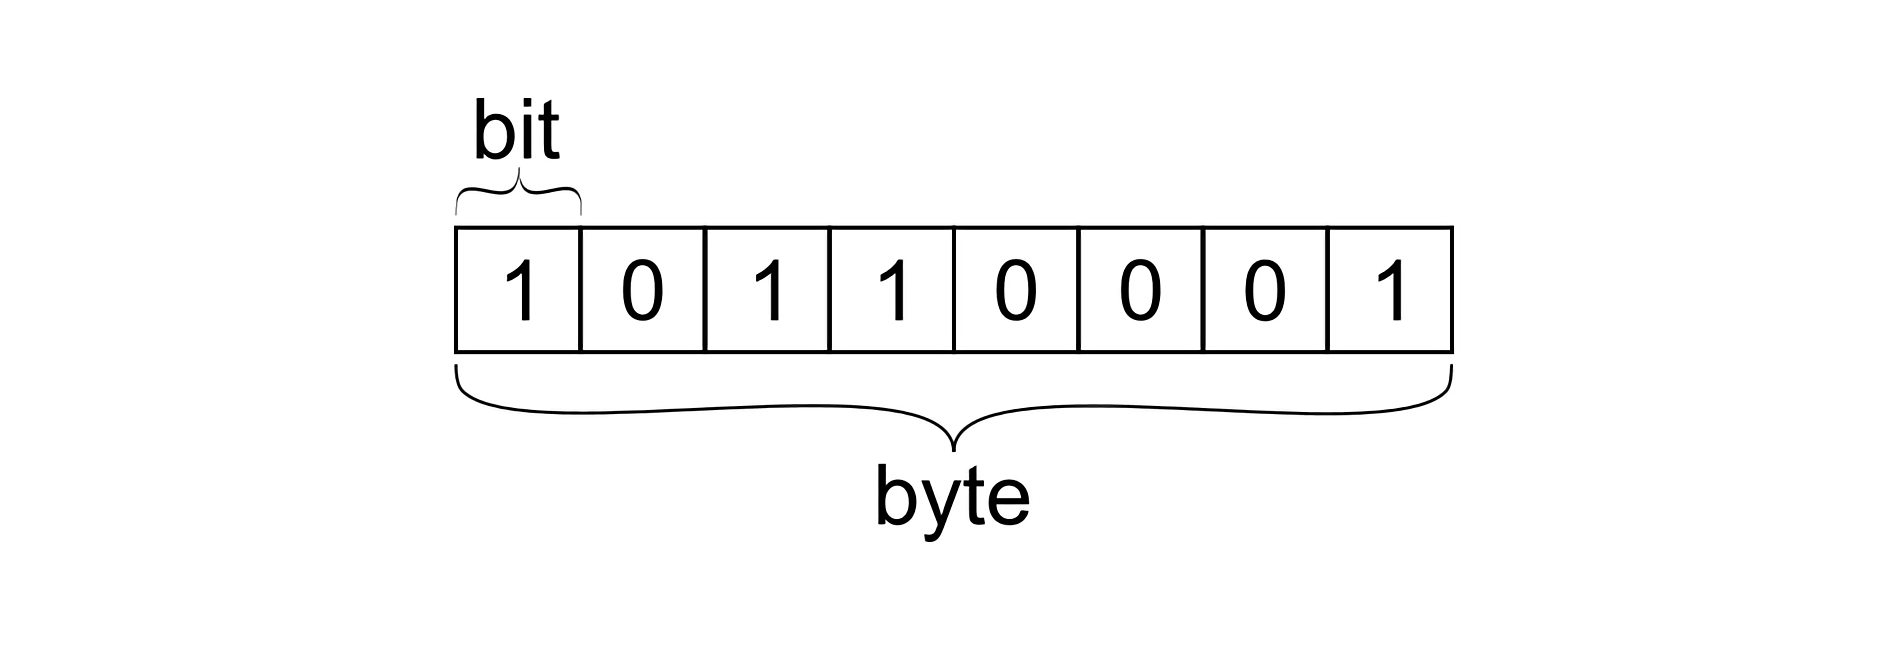
\includegraphics[width=0.7\linewidth]{Figuras/Ch02/fig3}
\end{frame}


\begin{frame}{Código fonte do computador}
	\begin{block}{Byte}
		\begin{itemize}
			\item Para calcular a quantidade de possibilidades que um byte pode representar, basta fazer a seguinte conta:
			      \[ 2 \times2 \times2 \times2 \times2 \times2 \times2 \times2 = 2^{8} = 256 \]
			\item 8 bits geram 256 números binários distintos, numa faixa de $ 0000\,0000 $ a $ 1111\,1111 $.
			\item Com bytes suficientes, podemos representar todas as letras (maiúsculas e minúsculas), sinais de pontuação, acentos, sinais especiais e, portanto, \textbf{todo tipo de caractere desejável}.
		\end{itemize}
	\end{block}

	%	\centering
	%	\includegraphics[width=0.7\linewidth]{Figuras/Ch02/fig}
\end{frame}


\begin{frame}{Código fonte do computador}
	\begin{block}{Sistema de codificação}
		\begin{itemize}
			\item Consiste em uma tabela, onde cada número binário representa um símbolo.
			\item Cada byte representa um caractere ou sinal.
			\item Visa prover comunicação entre o homem e o computador.
			\item Um padrão clássico é o \textbf{ASCII} (Código Padrão Americano para Troca de Informação).
			      %			\item Sistema decimal (0 a 9) $ \iff $ Sistema binário (0 e 1).
		\end{itemize}
	\end{block}

	%	\centering
	%	\includegraphics[width=0.7\linewidth]{Figuras/Ch02/fig}
\end{frame}


\begin{frame}{Código fonte do computador}
	\centering
	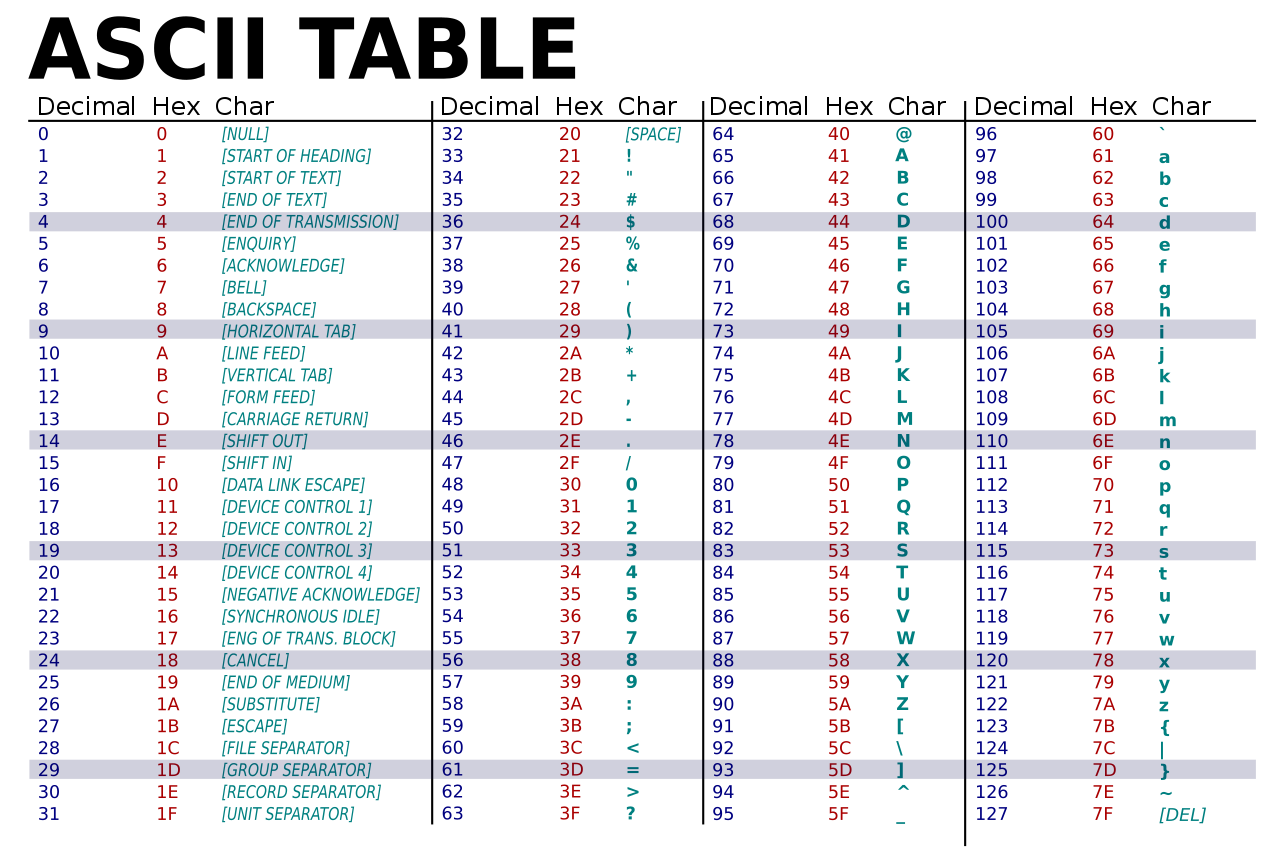
\includegraphics[width=0.9\linewidth]{Figuras/Ch02/fig2}
\end{frame}


\begin{frame}{Unidades de medida}
	\begin{block}{}
		\begin{itemize}
			\item Para facilitar a compreensão humana da capacidade de armazenamento, processamento e manipulação de dados nos computadores, usamos unidades de medida.
		\end{itemize}
	\end{block}

	\bigskip

	\centering
	\begin{tabular}{ccc}
		\toprule
		\SI{1}{\byte}      & \SI{8}{\bit}          & Aproximadamente um caractere             \\
		\SI{1}{\kilo\byte} & \SI{1024}{\byte}      & Aproximadamente mil caracteres           \\
		\SI{1}{\mega\byte} & \SI{1024}{\kilo\byte} & Aproximadamente um milhão de caracteres  \\
		\SI{1}{\giga\byte} & \SI{1024}{\mega\byte} & Aproximadamente um bilhão de caracteres  \\
		\SI{1}{\tera\byte} & \SI{1024}{\giga\byte} & Aproximadamente um trilhão de caracteres \\ \bottomrule
	\end{tabular}

	%	\centering
	%	\includegraphics[width=0.7\linewidth]{Figuras/Ch02/fig}
\end{frame}


\begin{frame}{Placa-mãe (\textit{Motherboard})}
	\begin{block}{}
		\begin{itemize}
			\item Placa de circuito impresso que \textbf{aloja o processador} e contém \textbf{encaixes} (slots) para a conexão dos demais componentes de entrada, saída e armazenamento.
			\item Responsável por \textbf{interconectar} cada um dos componentes do computador.
			%			\item Qualidade do computador pode ser avaliada pela qualidade e desempenho da placa-mãe.
			\item De acordo com suas especificações, define o quanto esse computador pode evoluir, ou seja, o quanto seu desempenho pode ser melhorado.
			\item \textit{Upgrade}: Em informática, o termo é usado para designar a ação de \textbf{melhorar os componentes} do computador, através da troca ou adição dos mesmos.
		\end{itemize}
	\end{block}
\end{frame}


\begin{frame}{Placa-mãe (\textit{Motherboard})}
	\begin{minipage}{0.49\linewidth}
		\centering
		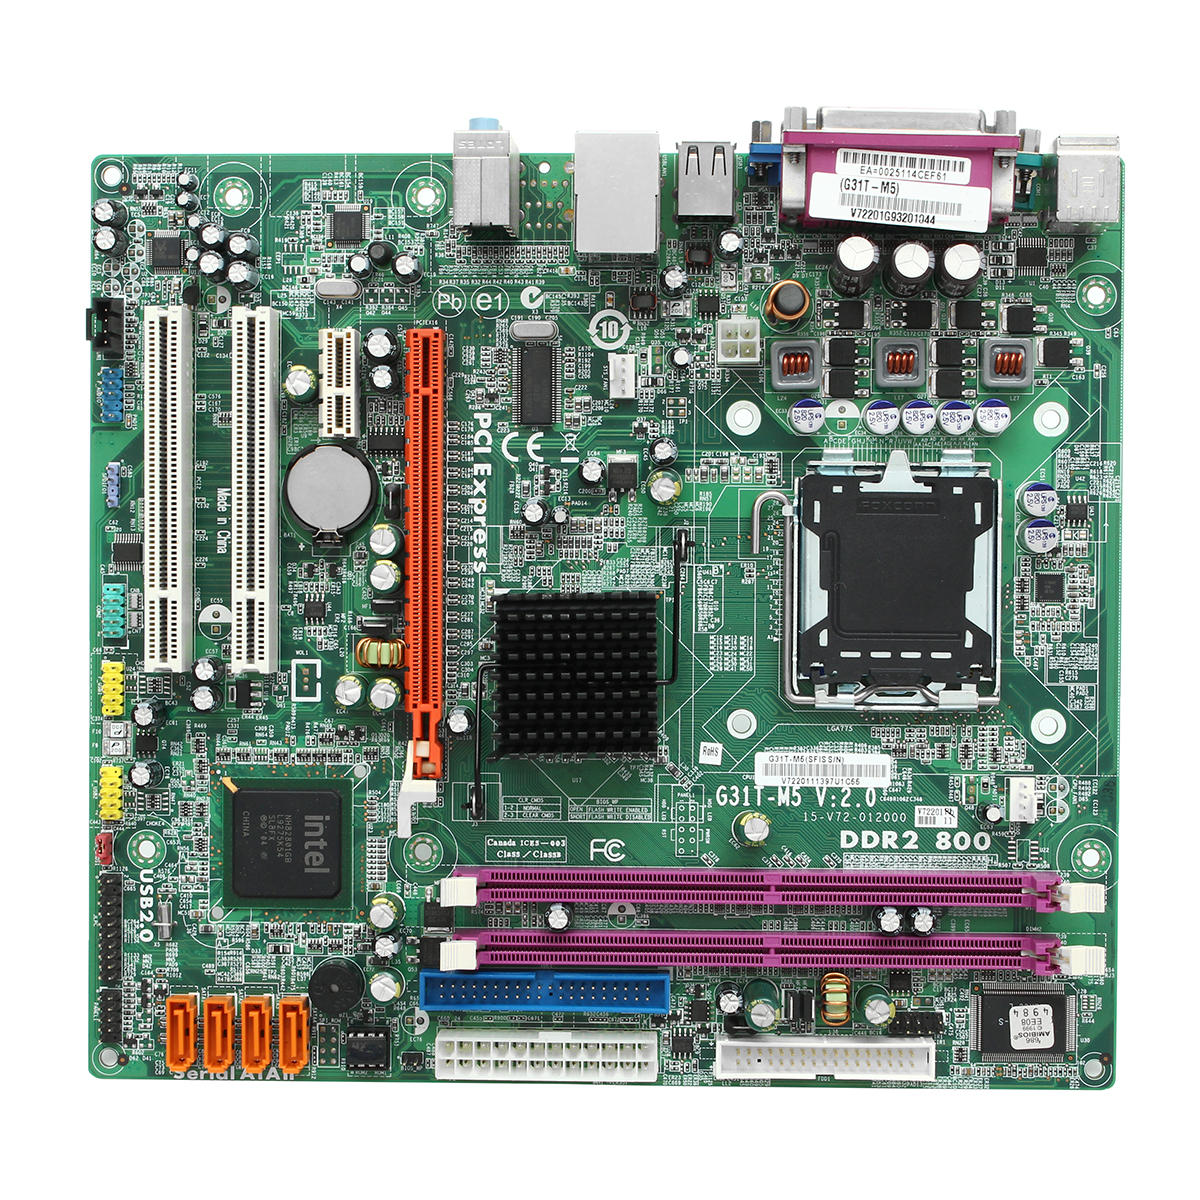
\includegraphics[width=1\linewidth]{Figuras/Ch02/fig4}
	\end{minipage}\hfill
	\begin{minipage}{0.49\linewidth}
		\centering
		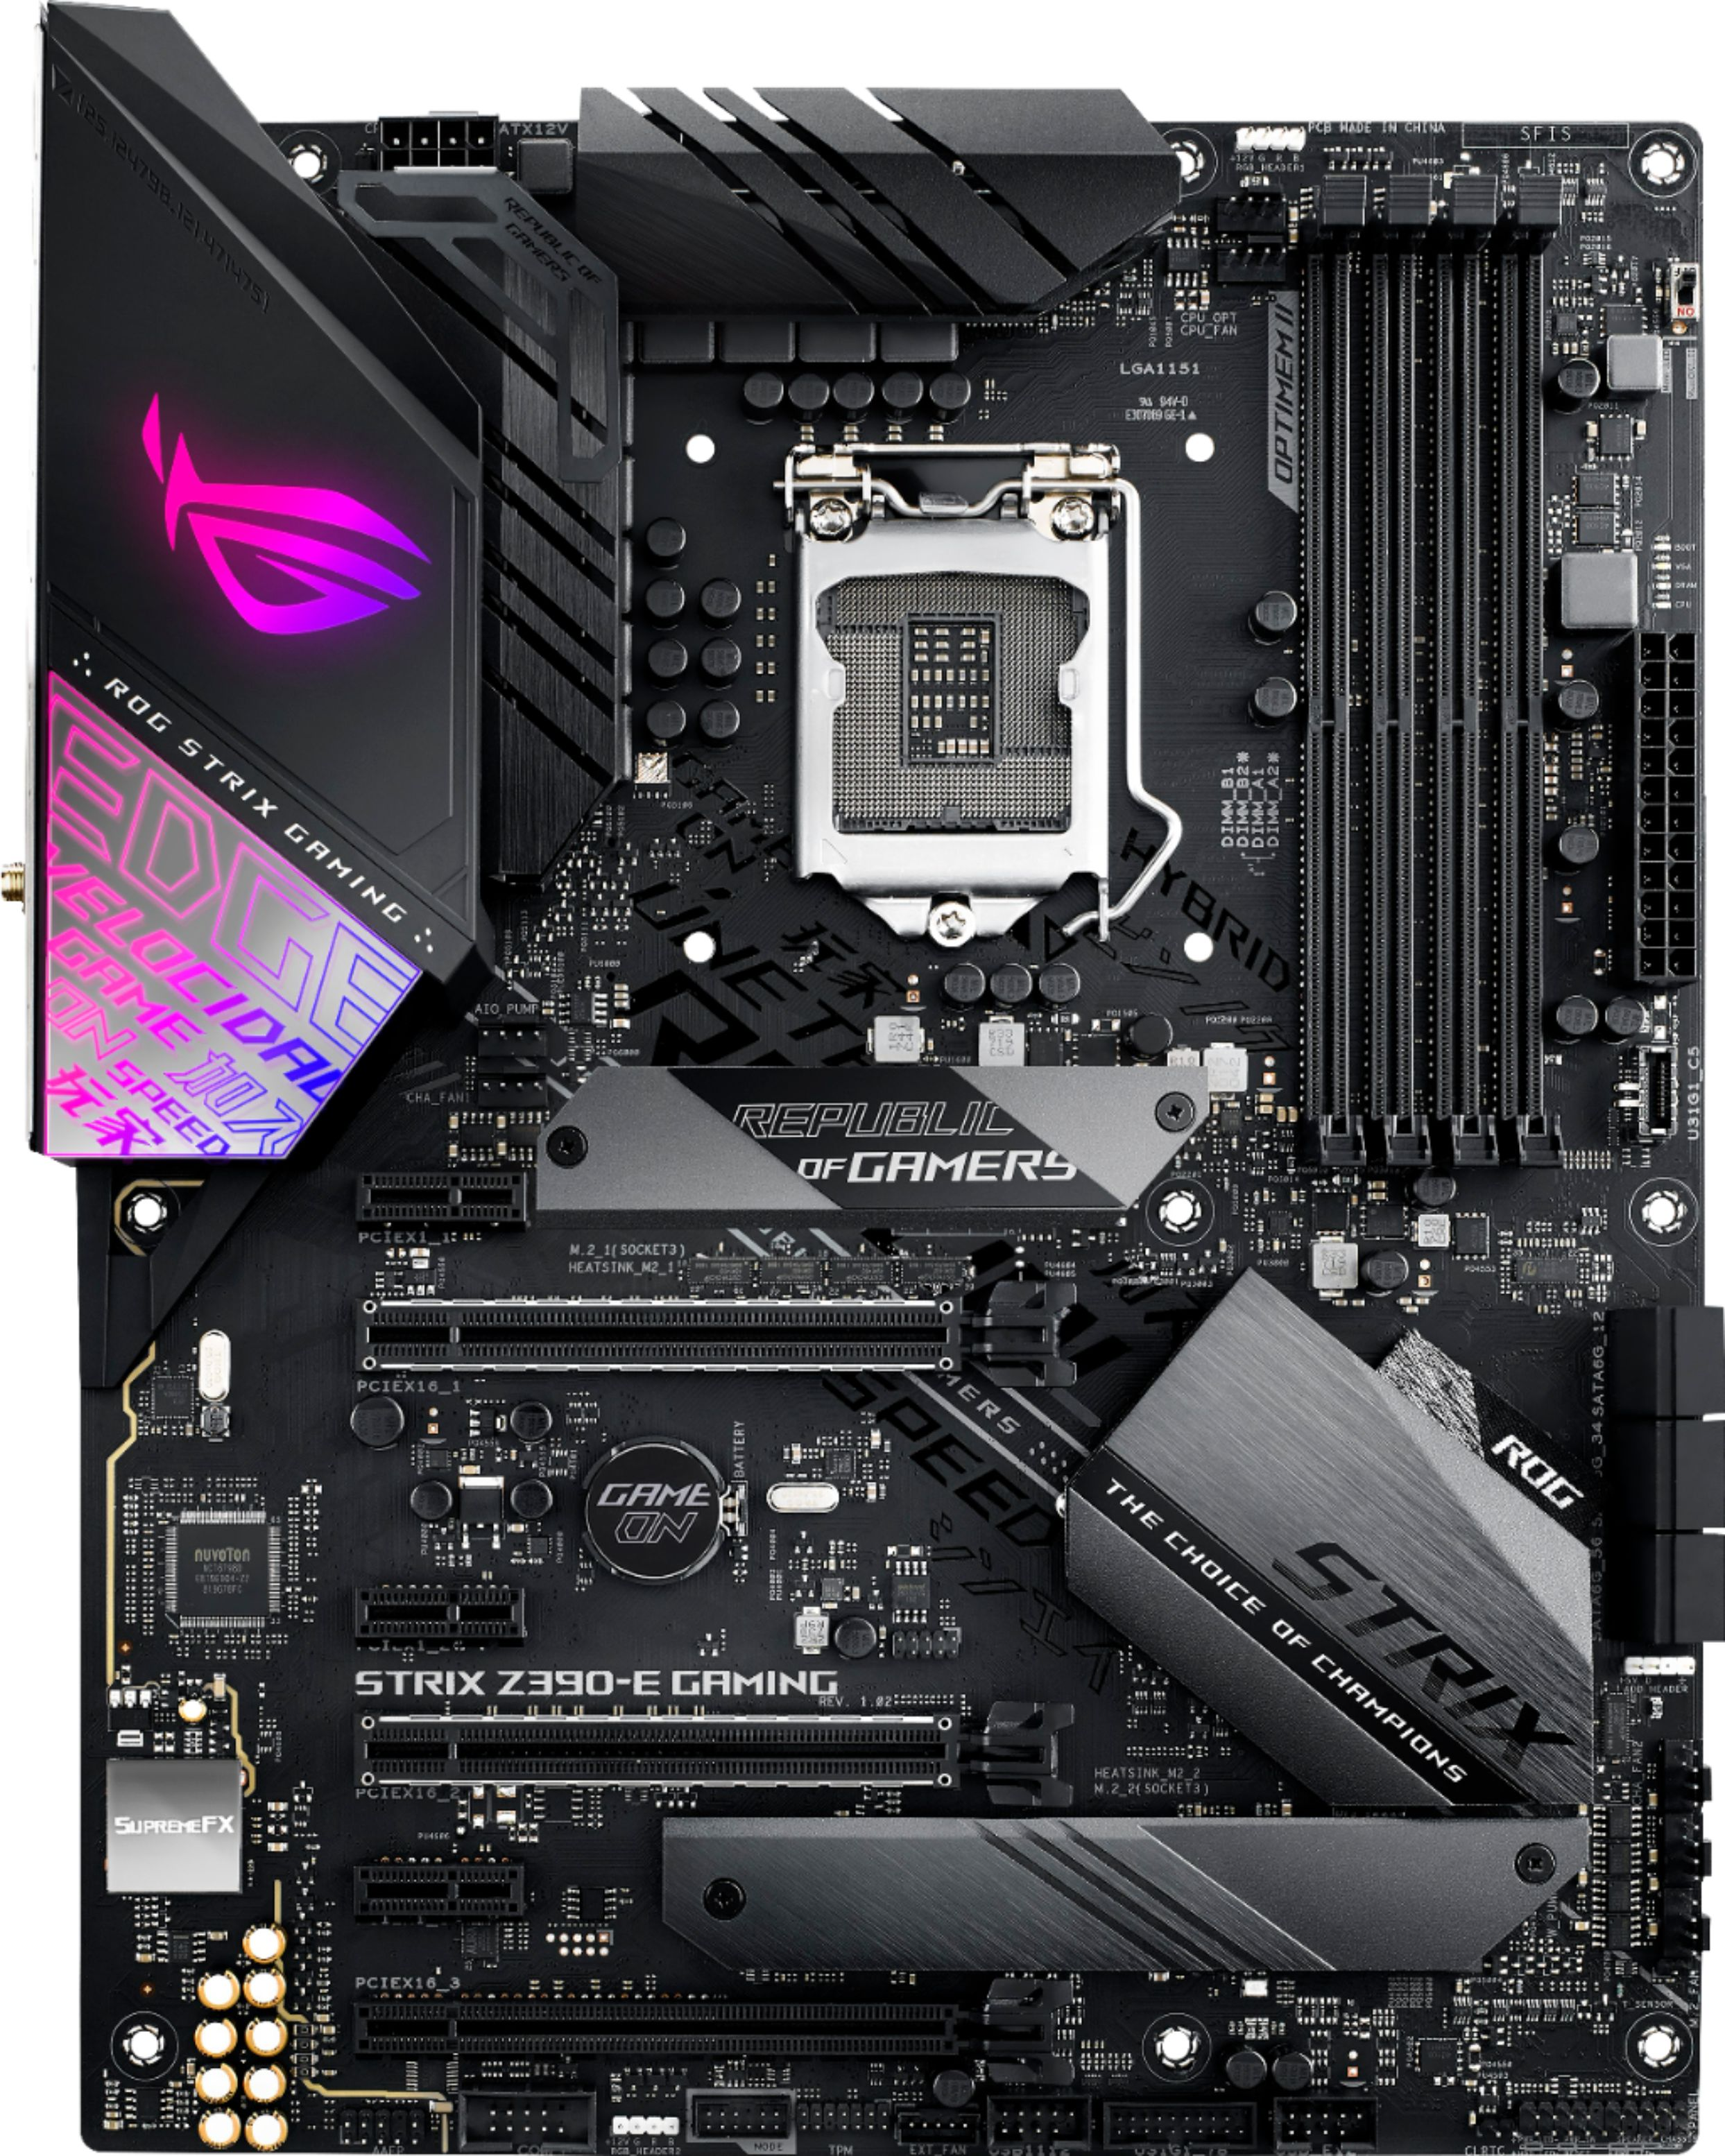
\includegraphics[width=1\linewidth]{Figuras/Ch02/fig5}
	\end{minipage}
\end{frame}


\begin{frame}{Placa-mãe (\textit{Motherboard})}
	\centering
	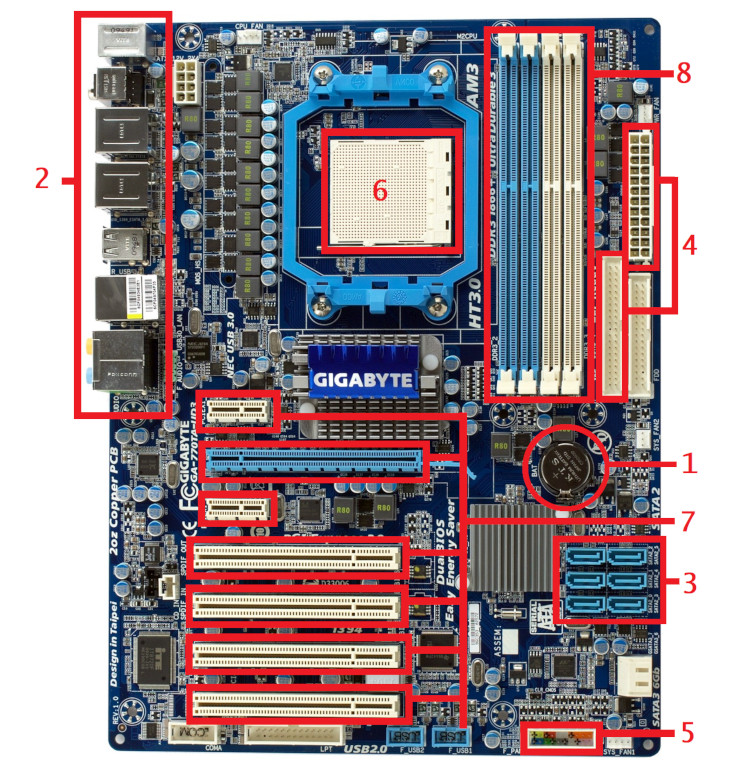
\includegraphics[width=0.6\linewidth]{Figuras/Ch02/fig6}
\end{frame}


\begin{frame}{Placa-mãe (\textit{Motherboard})}
	\begin{block}{}
		\begin{enumerate}
			\item BIOS e CMOS: a BIOS é a configuração básica que rege o funcionamento da placa mãe, e a CMOS é uma pequena bateria que mantém as configurações do usuário salvas, além de dados como hora e data;
			\item I/Os da placa;
			\item conectores IDE e SATA;
			\item conectores de energia;
			\item I/Os frontais (para USBs e outras coisas na frente do gabinete);
			\item socket do processador;
			\item slots para cartões de expansão (PCI's e PCIe's);
			\item slots de memória RAM.
		\end{enumerate}
	\end{block}
\end{frame}


\begin{frame}{Placa-mãe (\textit{Motherboard})}
	\begin{block}{Interfaceamento}
		\begin{itemize}
			\item Para que as peças do computador se \textbf{comuniquem} com o sistema operacional, e também para fazer os programas conversarem com os \textbf{periféricos}, como mouse e teclado, precisamos de um \textbf{kernel}.
		\end{itemize}
	\end{block}
	
	\centering
	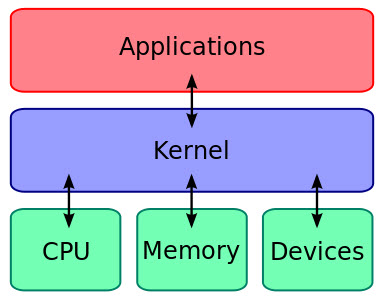
\includegraphics[width=0.6\linewidth]{Figuras/Ch02/fig0}
\end{frame}


\begin{frame}{Placa-mãe (\textit{Motherboard})}
	\begin{block}{Interfaceamento}
		\begin{itemize}
			\item Enquanto ``liga'', o Windows está carregando seu kernel.
		\end{itemize}
	\end{block}
	
	\centering
	
\includegraphics[width=1\linewidth]{Figuras/Ch02/fig0.1}
\end{frame}


\begin{frame}{Placa-mãe (\textit{Motherboard})}
	\begin{block}{Especificações úteis}
		\begin{itemize}
			\item Podemos observar algumas especificações úteis na hora de \textbf{comparar} diferentes placas-mãe.
			\item A \textbf{velocidade do \textit{bus}}, por exemplo, ou sua \textbf{capacidade máxima de memória}, além de especificações de outros componentes embutidos na própria placa, e até capacidade de aceitar certos dispositivos (entradas para M.2 ou PCI-e).
			\item Essas especificações determinam a velocidade máxima de operação dos outros componentes do computador, e, portanto, a capacidade total da operação do computador.
			\item Caso não nos atentemos a esses detalhes, pode ocorrer o fenômeno do \textbf{gargalo} (\textit{bottleneck}): a \textbf{limitação física} de um dos componentes acaba \textbf{limitando a ação} dos outros.
		\end{itemize}
	\end{block}
\end{frame}


\begin{frame}{Processador (CPU)}
	\begin{block}{}
		\begin{itemize}
			\item CPU (\textit{Central Processing Unit}) – Unidade Central de Processamento: chip eletrônico com milhões de componentes microscópicos, chamados \textbf{transistores}.
			\item Os transistores são capazes de realizar \textbf{operações simples}, que se resumem a \textbf{manipulações de dados}.
			\item Ele é a parte ``central'' de um computador, funcionando como uma espécie de \textbf{cérebro} da máquina, realizando \textbf{cálculos}, completando \textbf{tarefas}, realizando \textbf{transformações}.
			\item Todas essas tarefas são \textbf{manipulações de dados}, em essência, e estudamos algumas técnicas utilizadas para computações em \textbf{eletrônica digital}.
		\end{itemize}
	\end{block}
\end{frame}


\begin{frame}{Componentes do processador}
	\begin{block}{Unidade de Controle (UC)}
		\begin{itemize}
			\item É a parte do processador responsável pelo \textbf{controle das ações a serem realizadas} pelo mesmo.
			\item Faz o papel de \textbf{gerente} do processador, \textbf{indica} e \textbf{fiscaliza} o que deve ser feito e \textbf{comanda} os demais componentes do processador.
		\end{itemize}
	\end{block}

	%	\centering
	%	\includegraphics[width=0.7\linewidth]{Figuras/Ch02/fig}
\end{frame}


\begin{frame}{Componentes do processador}
	\begin{block}{Unidade Lógica Aritmética (ULA)}
		\begin{itemize}
			\item É a parte que \textbf{executa} as instruções \textbf{lógicas} e \textbf{aritméticas} dos programas.
			\item Faz o papel do trabalhador que executa as \textbf{ordens} do gerente.
		\end{itemize}
	\end{block}

	\begin{block}{Registradores}
		\begin{itemize}
			\item São \textbf{memórias internas} do processador utilizadas para auxiliar a UC e a ULA no \textbf{controle} e na \textbf{execução} das instruções.
			\item Armazenam poucos dados, mas são memórias de \textbf{grande velocidade de acesso} por serem internas ao processador.
		\end{itemize}
	\end{block}
\end{frame}


\begin{frame}{Componentes do processador}
	\centering
	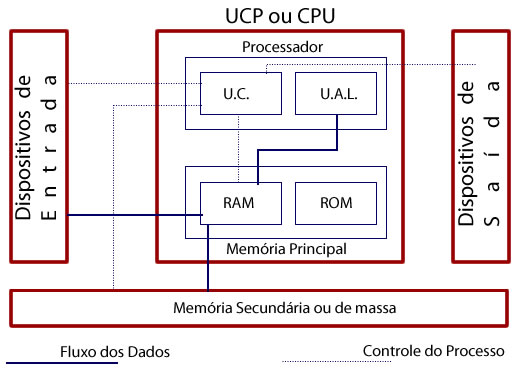
\includegraphics[width=1\linewidth]{Figuras/Ch02/fig7}
\end{frame}


\begin{frame}{Processador (CPU)}
	\begin{block}{Especificações úteis}
		\begin{itemize}
			\item Antigamente, era muito útil olhar algumas especificações dos processadores, como \textbf{Clock}, \textbf{TDP}, ou \textbf{número de núcleos}, porém, hoje em dia é uma ciência muito incerta, e essas especificações \textbf{não significam muita coisa}.
			\item Como resumo, o \textit{Clock} é a medida de quantas operações o processador faz, por unidade de tempo (por isso é medido em Hertz (\si{\hertz})).
			\item O TDP é uma medida de \textbf{eficiência energética do componente}, e não está disponível só para processadores (nas placas de vídeo, por exemplo, é uma especificação \textbf{importantíssima}), e é medido em Watts (\si{\watt}).
			\item O número de núcleos representa a quantidade de operações que podem ser executadas \textbf{simultaneamente}, e ainda existem núcleos \textbf{físicos} e \textbf{virtuais}.
		\end{itemize}
	\end{block}
\end{frame}


\begin{frame}{Memórias}
	\begin{block}{}
		\begin{itemize}
			\item Já vimos que a memória é essencial para o computador funcionar. De fato, não existe computador que funcione sem memória.
			\item Essencialmente, há dois tipos de memória:
			      \begin{itemize}
				      \item\normalsize \textbf{principal:} auxilia o processador no processamento de dados;
				      \item\normalsize \textbf{secundária:} armazenamento definitivo de informações.
			      \end{itemize}
		\end{itemize}
	\end{block}

	%	\centering
	%	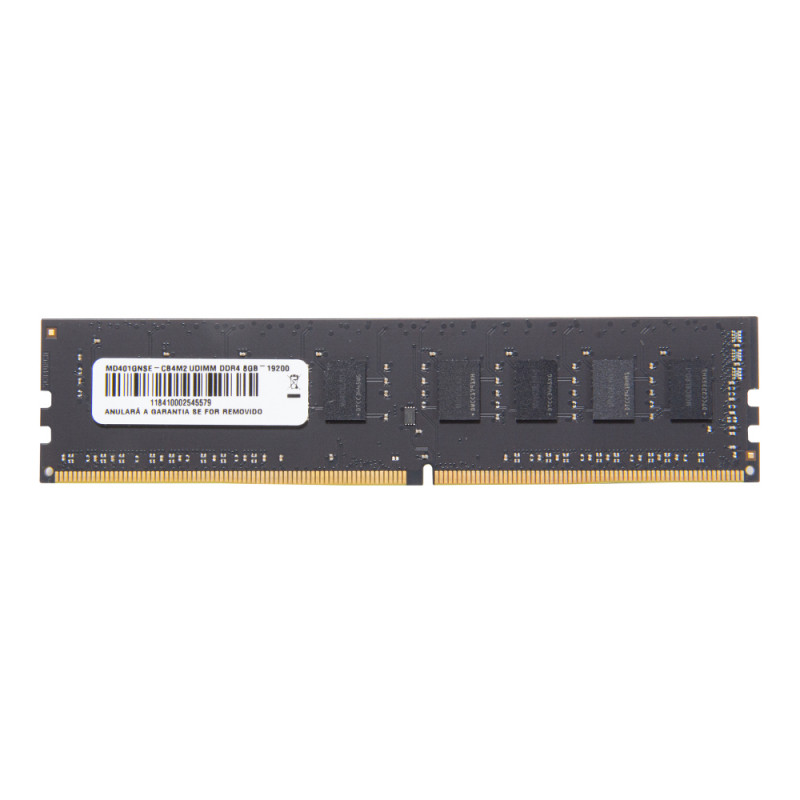
\includegraphics[width=0.7\linewidth]{Figuras/Ch02/fig8.1}
\end{frame}


\begin{frame}{Memórias}
	\begin{block}{Memória principal}
		\begin{itemize}
			\item Os programas em execução no computador devem estar carregados na memória \textbf{principal}.
			\item Se o processador precisar de alguma informação localizada na memória secundária, então a informação deve ser \textbf{recuperada} e \textbf{armazenada na memória principal}.
		\end{itemize}
	\end{block}

	\begin{minipage}{0.49\linewidth}
		\centering
		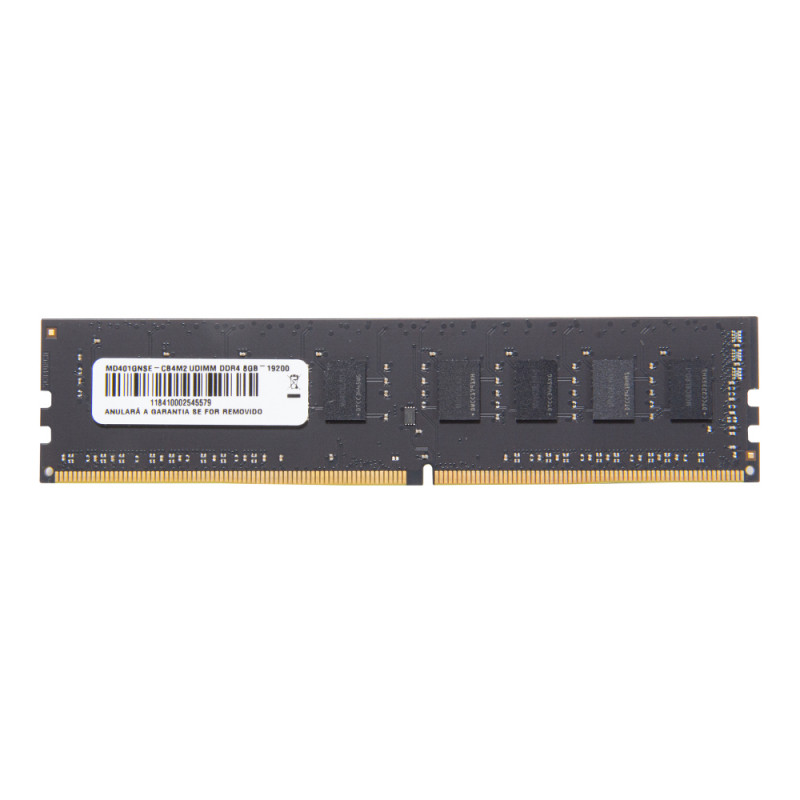
\includegraphics[width=1\linewidth]{Figuras/Ch02/fig8.1}
	\end{minipage}
	\hfill
	\begin{minipage}{0.49\linewidth}
		\centering
		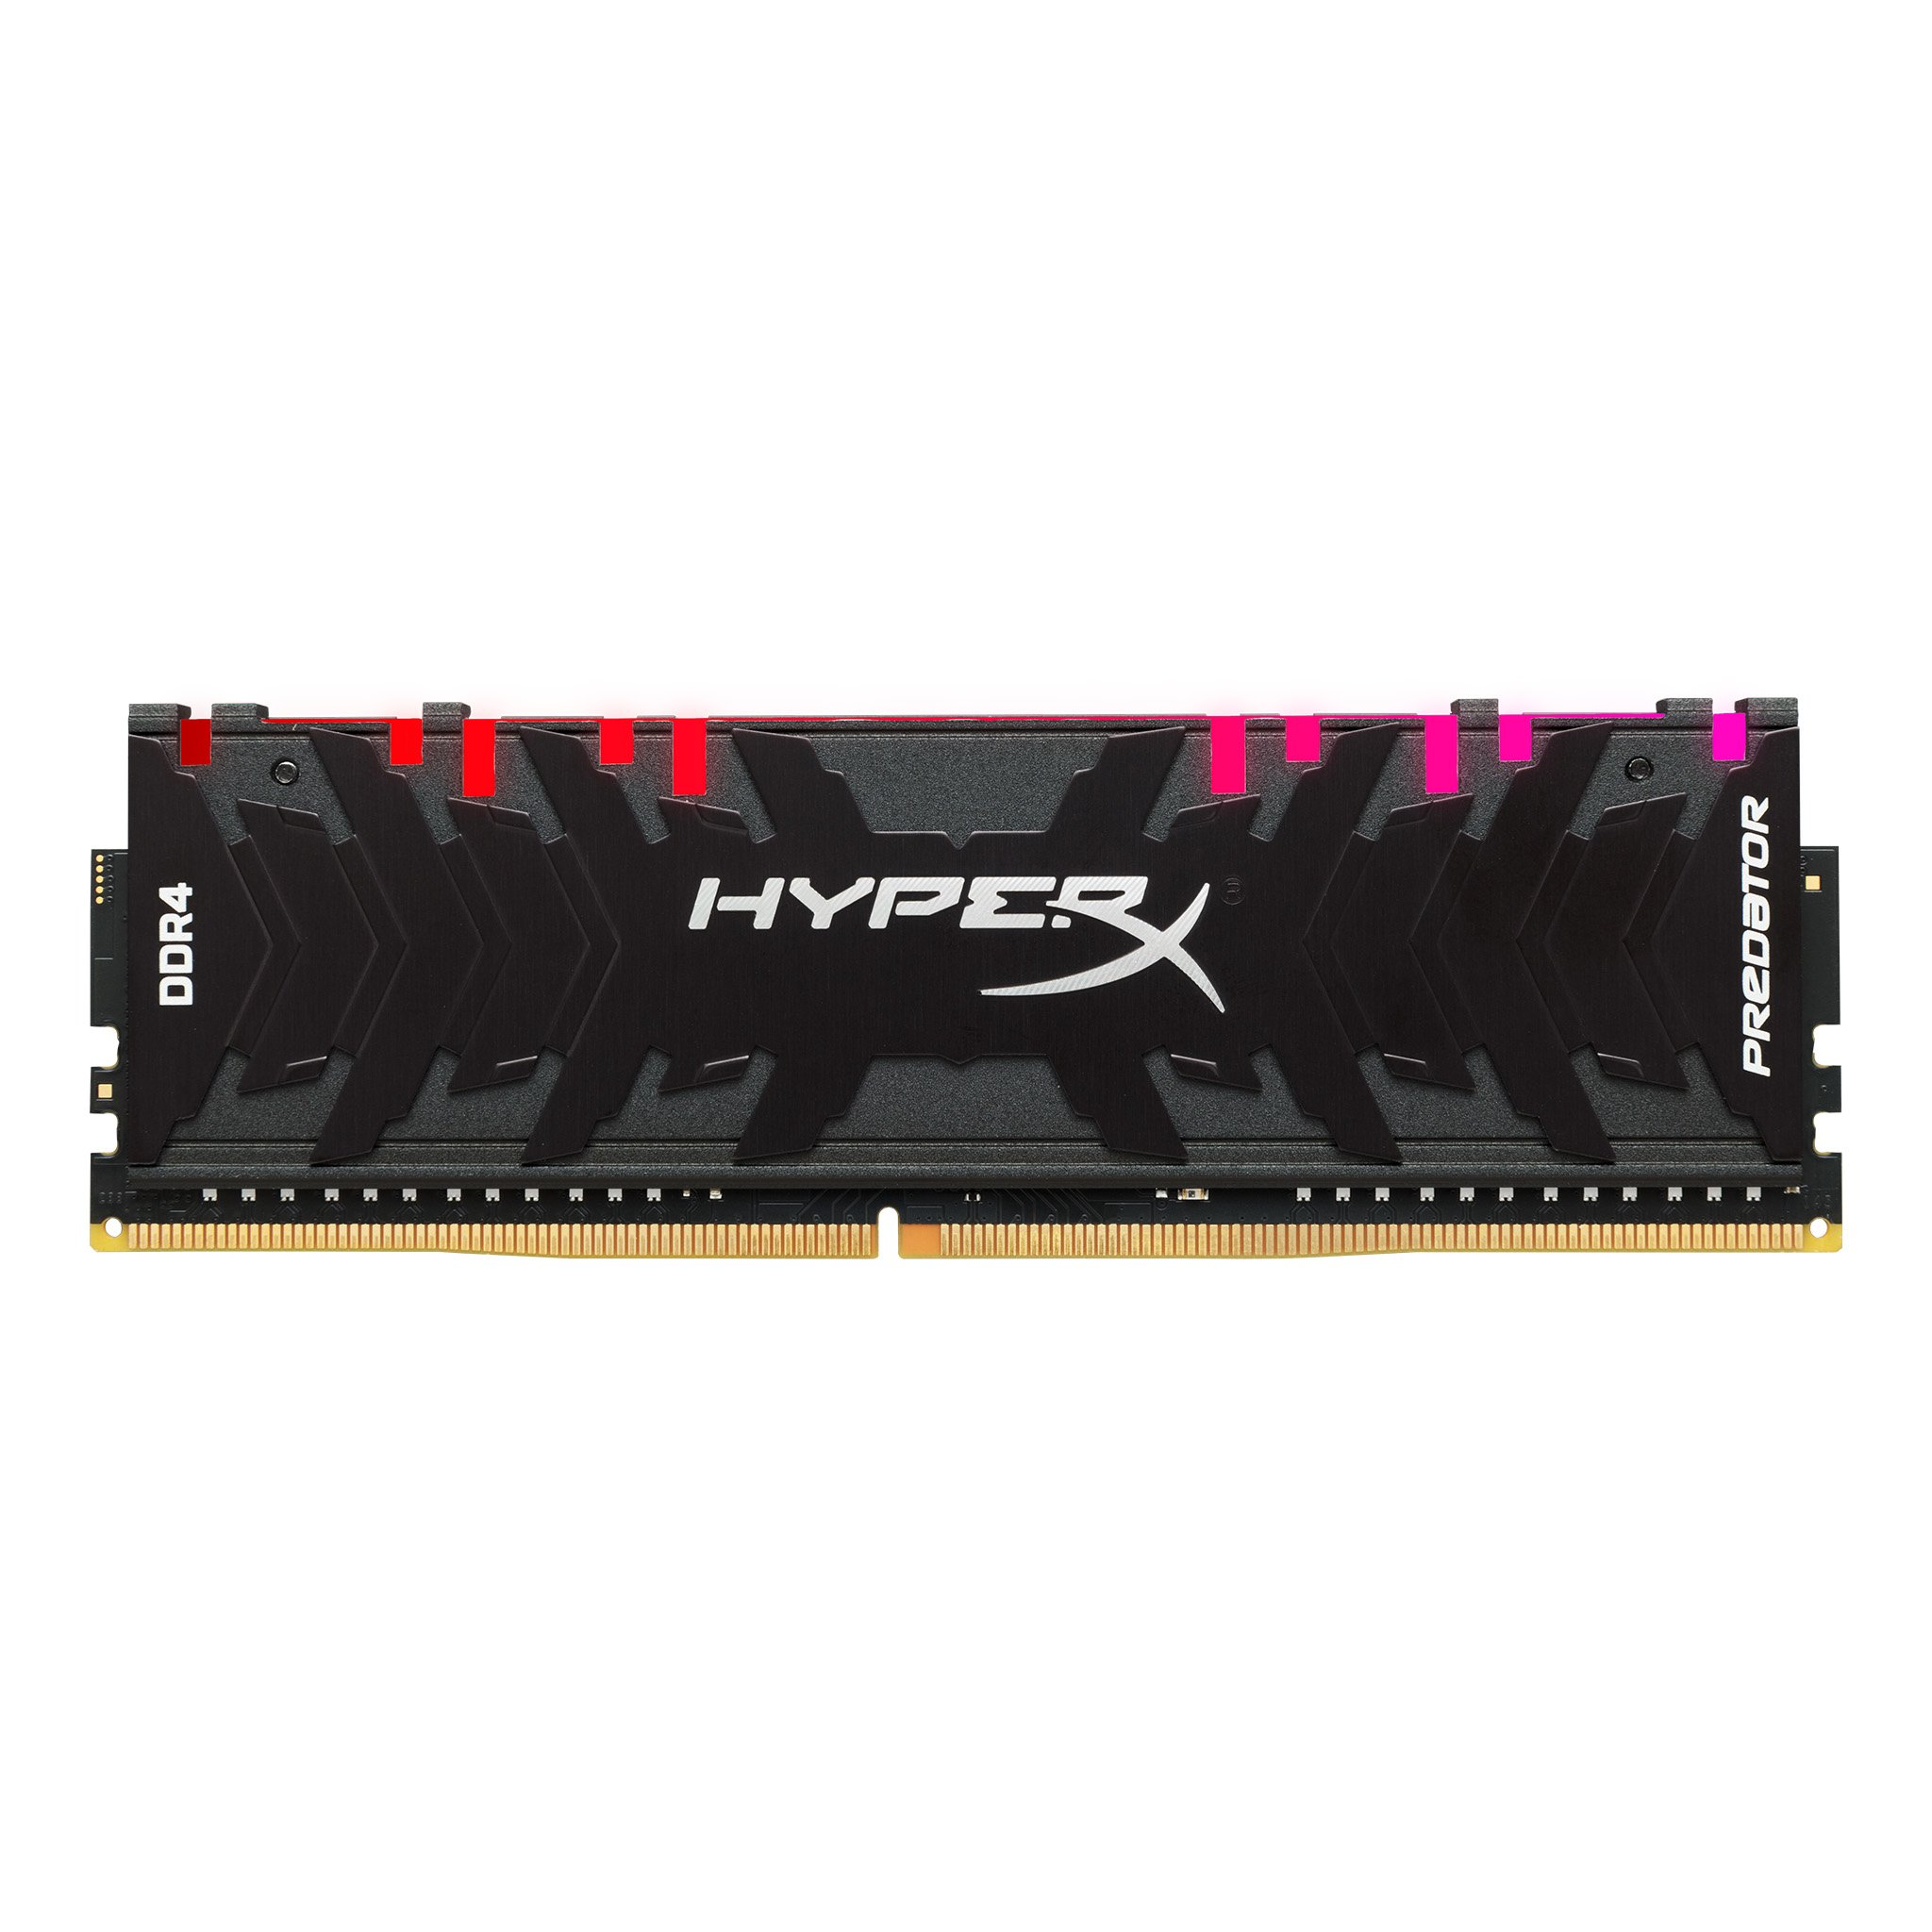
\includegraphics[width=1\linewidth]{Figuras/Ch02/fig8.2}
	\end{minipage}
\end{frame}


\begin{frame}{Memórias}
	\begin{block}{Especificações úteis}
		\begin{itemize}
			\item A memória de armazenamento, que pode ser em forma de discos ou cartões, pode ter sua eficiência estimada pelas \textbf{velocidades de leitura} e de \textbf{escrita}, que medem a \textbf{rapidez} com que podemos \textbf{acessar} e \textbf{gravar} informações no disco.
			\item Já a memoria principal, chamada de \textbf{RAM}, tem sua velocidade medida pela \textbf{frequência de operação} (similar à frequência do processador -- clock) e pela \textbf{latência CAS}, que mede o tempo necessário para a memória agir sob um comando de leitura.
			\item A \textbf{capacidade} de ambas é geralmente o fator principal a ser considerado na compra, embora para o armazenamento as velocidades sejam mais importantes, em geral.
		\end{itemize}
	\end{block}

	%	\centering
	%	\includegraphics[width=0.7\linewidth]{Figuras/Ch02/fig}
\end{frame}


\begin{frame}{Memórias}
	\begin{block}{Memória secundária}
		\begin{itemize}
			\item Um HDD (\textit{Hard-Disk Drive}) é um dos tipos \textbf{mais antigos} de memória secundária, que consiste num ``disco rígido'' que lê e grava dados em discos de metal usando uma paleta com um laser e um ímã na ponta.
			\item Já o SSD (\textit{Solid-State Drive}) não possui partes móveis, consistindo em vários chips, similares aos de uma memória RAM, sendo muito mais \textbf{rápido, leve, e silencioso} do que o HD.
		\end{itemize}
	\end{block}

	\centering
	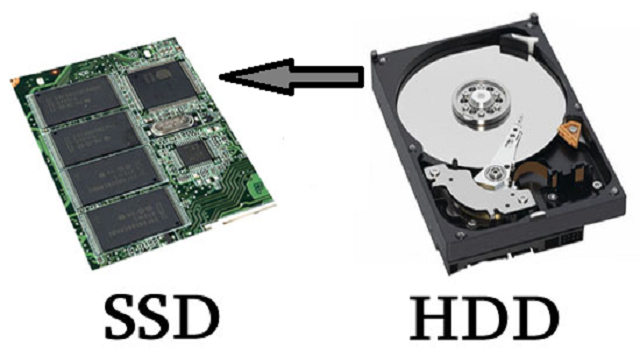
\includegraphics[width=0.6\linewidth]{Figuras/Ch02/fig8}
\end{frame}


\begin{frame}{Fonte de Alimentação}
	\begin{block}{}
		\begin{itemize}
			\item Tem como finalidade receber a tensão da rede elétrica (\SI{110}{\volt} ou \SI{220}{\volt} em corrente alternada) e gerar tensões em corrente contínua necessárias ao funcionamento das placas do computador.
			\item A tensão da tomada, com frequência, precisa de \textbf{diversos tratamentos} para ser utilizada, e é isso que a fonte faz.
		\end{itemize}
	\end{block}

	\centering
	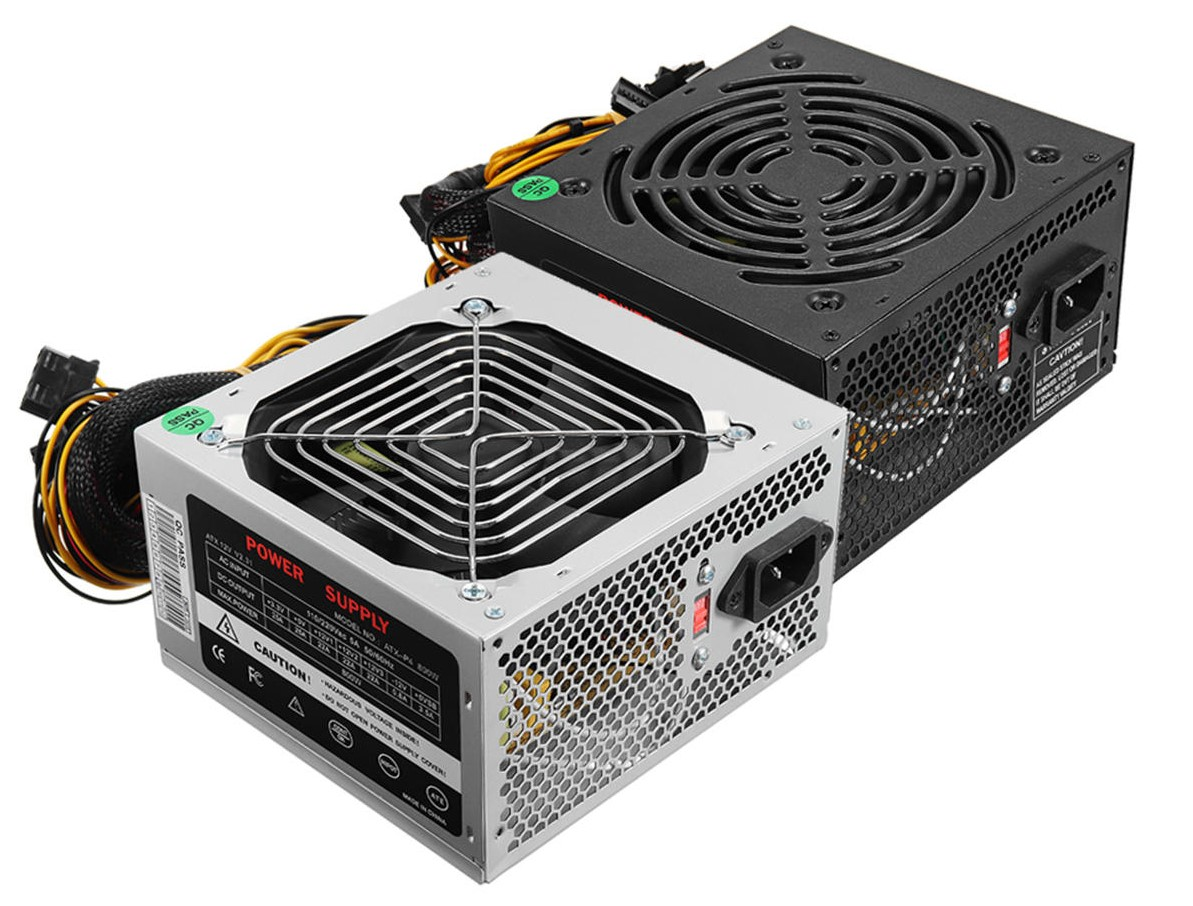
\includegraphics[width=0.55\linewidth]{Figuras/Ch02/fig9}
\end{frame}


\begin{frame}{Estabilizador}
	\begin{block}{}
		\begin{itemize}
			\item Equipamento que protege o computador de \textbf{oscilações} na rede elétrica que, em geral, acontecem durante \textbf{tempestades}.
			\item Serve também para \textbf{atenuar interferências}, \textbf{quedas de voltagem} e \textbf{outras anomalias} na rede elétrica.
		\end{itemize}
	\end{block}

	\medskip

	\centering
	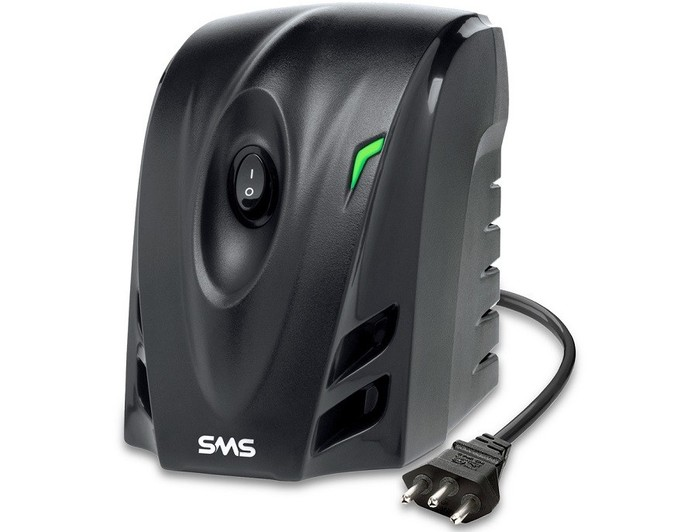
\includegraphics[width=0.55\linewidth]{Figuras/Ch02/fig10}
\end{frame}


\begin{frame}{No-break}
	\begin{block}{}
		\begin{itemize}
			\item Além de possuir mesmas funções do estabilizador, \textbf{evita que o computador desligue} em caso de falta total de energia elétrica.
			\item Possui baterias que mantém o funcionamento de um computador por algum período de tempo.
		\end{itemize}
	\end{block}

	\centering
	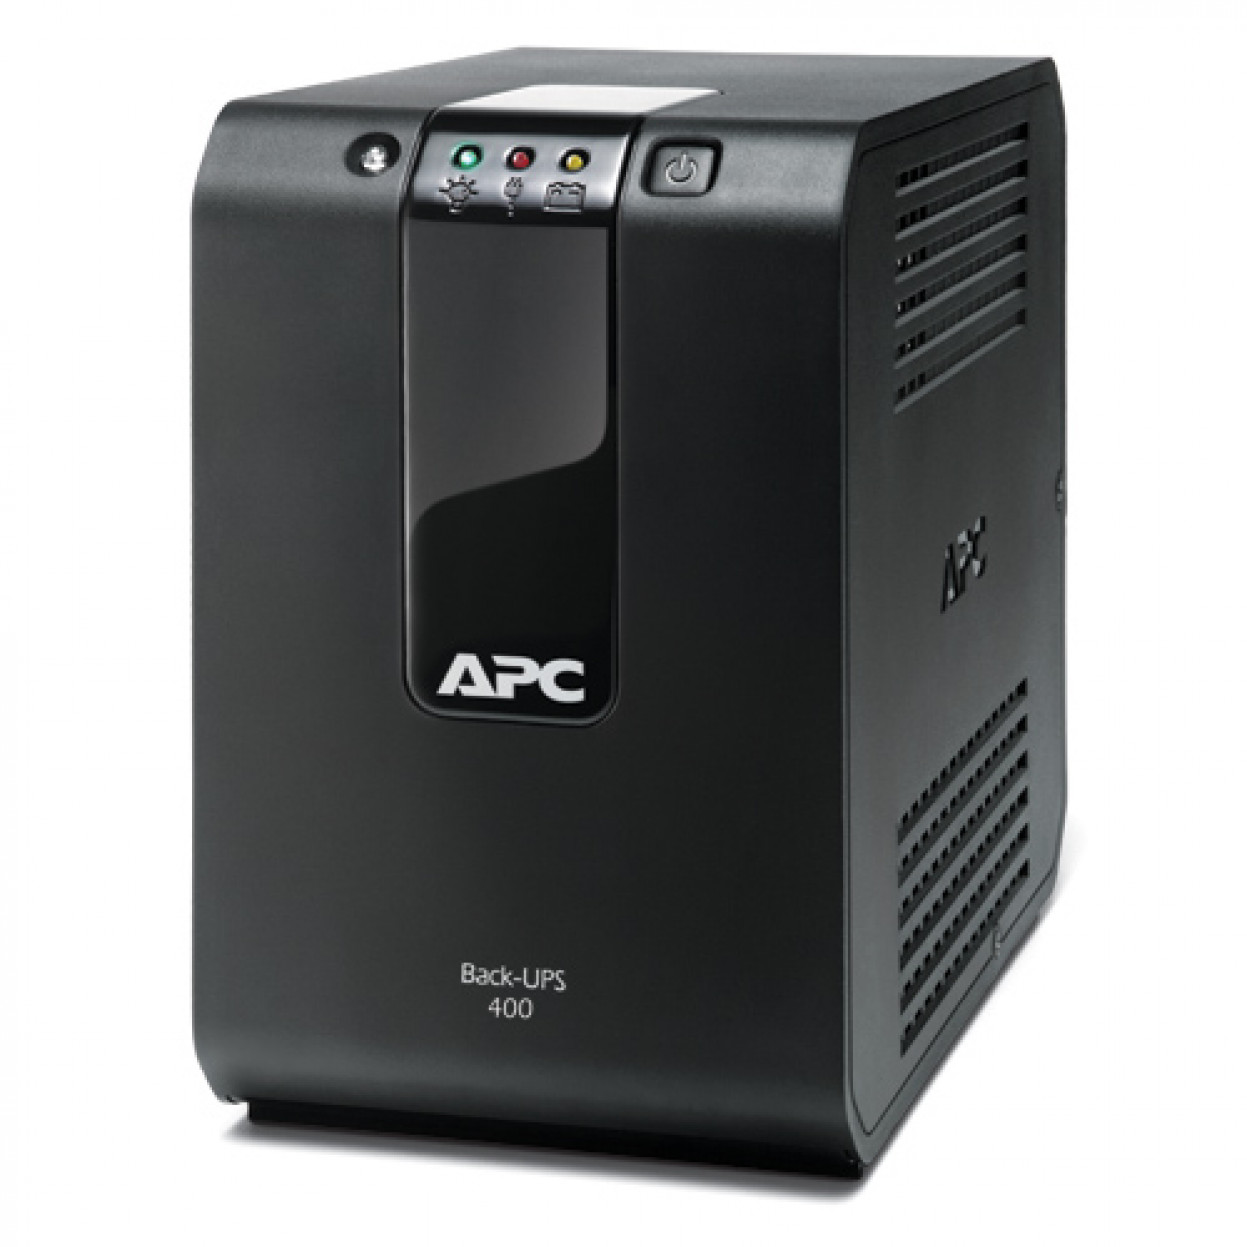
\includegraphics[width=0.45\linewidth]{Figuras/Ch02/fig11}
\end{frame}


\begin{frame}{Mouse}
	\begin{block}{}
		\begin{itemize}
			\item É um dispositivo de entrada que detecta deslocamento relativo (movimentos).
			\item Ele também permite algumas entradas, como os cliques, e rolar a tela, mas alguns modelos possuem outras funcionalidades.
		\end{itemize}
	\end{block}

	\begin{minipage}{0.49\linewidth}
		\centering
		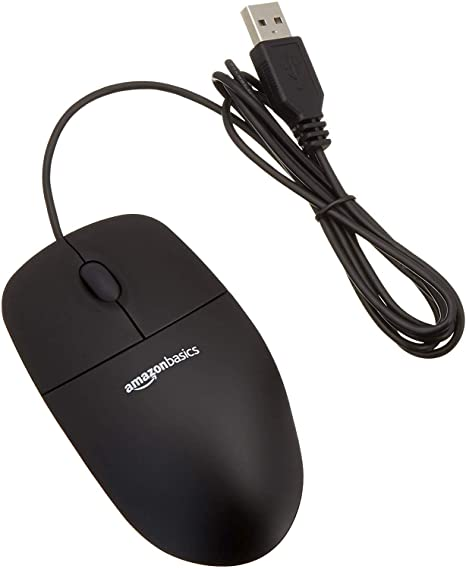
\includegraphics[width=0.7\linewidth]{Figuras/Ch02/fig12}
	\end{minipage}
	\hfill
	\begin{minipage}{0.49\linewidth}
		\centering
		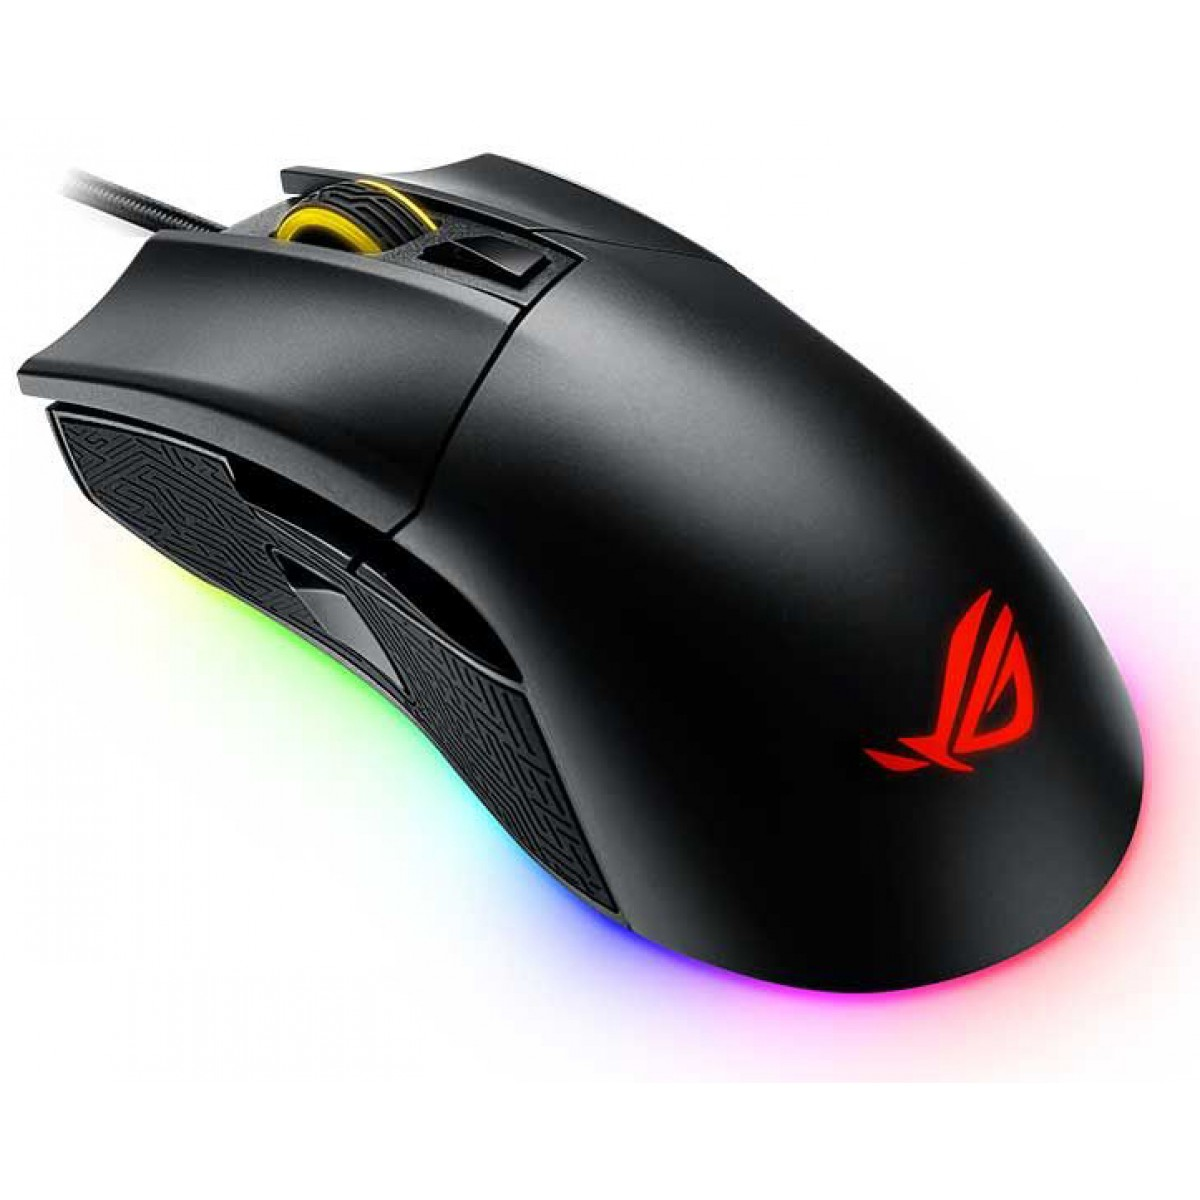
\includegraphics[width=0.7\linewidth]{Figuras/Ch02/fig13}
	\end{minipage}
\end{frame}


\begin{frame}{Mouse}
	\begin{block}{Cursor do Mouse}
		\begin{itemize}
			\item O cursor do mouse é uma representação de onde o usuário quer interagir com a máquina, como se fosse ``sua mão'', apertando botões, e fazendo diversas tarefas.
			\item A depender de qual elemento se encontra abaixo do cursor ou do que o computador estiver executando no momento, temos \textbf{representações diferentes}.
		\end{itemize}
	\end{block}

	\centering
	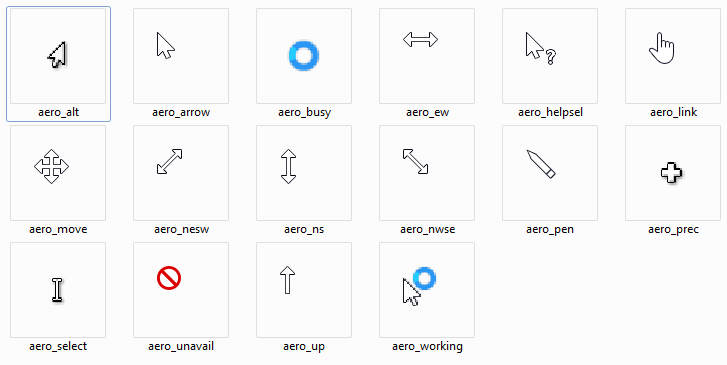
\includegraphics[width=0.6\linewidth]{Figuras/Ch02/fig14}
\end{frame}


\begin{frame}{Cursor do Mouse}
	%	\begin{block}{}
	%		\begin{itemize}
	%			\item Selecionar itens ou clicar em botões (um clique) ou abrir pastas e arquivos ou executar programas (duplo clique).
	%			\item Computador está carregando algum programa ou arquivo ou executando uma ação demorada.
	%			\item Significa que o cursor encontra-se sobre algo clicável, como um link.
	%			Selecionar ou editar textos.
	%			\item Selecionar ou editar textos.
	%		\end{itemize}
	%	\end{block}

	\begin{minipage}{0.24\linewidth}
		\centering
		
\includegraphics[width=0.8\linewidth]{Figuras/Ch02/fig15}
	\end{minipage}\hfill
	\begin{minipage}{0.24\linewidth}
		\centering
		
\includegraphics[width=0.9\linewidth]{Figuras/Ch02/fig16}
	\end{minipage}\hfill
	\begin{minipage}{0.24\linewidth}
		\centering
		
\includegraphics[width=1\linewidth]{Figuras/Ch02/fig17}
	\end{minipage}\hfill
	\begin{minipage}{0.24\linewidth}
		\centering
		
\includegraphics[width=0.7\linewidth]{Figuras/Ch02/fig18}
	\end{minipage}

\end{frame}


\begin{frame}{Teclado}
	\begin{block}{}
		\begin{itemize}
			\item É um dispositivo de entrada de dados que possui várias ``teclas''.
			\item Cada uma delas representa um \textbf{caractere}, ou realiza uma \textbf{função específica}:
			      \begin{itemize}
				      \item\normalsize Shift: geralmente serve para deixar as letras em \textbf{maiúsculo} (ABCDE...), ou \textbf{alterar sua saída} (Shift+1 produz ``!'');

				            \smallskip

				      \item\normalsize Ctrl (Leia ``Control''): geralmente executa \textbf{atalhos} dentro de um programa (Ctrl+R recarrega a página do navegador);

				            \smallskip

				      \item\normalsize Alt: ativa as funcionalidades da \textbf{barra superior} do programa;

				            \smallskip

				      \item\normalsize Win (símbolo do Windows no teclado): executa atalhos relacionados ao \textbf{sistema operacional} (Win+L bloqueia o computador).
			      \end{itemize}
			      As teclas anteriores podem ser utilizadas \textbf{em conjunto} para termos outros atalhos (Ctrl+Shift+N cria uma nova pasta no Explorer).
		\end{itemize}
	\end{block}
\end{frame}


\begin{frame}{Teclado}
	\begin{block}{}
		\begin{itemize}
			\item Temos, ainda, mais outras teclas de função comuns:
			      \begin{itemize}
				      \item\normalsize F1, F2, F3 ... F12: realizam \textbf{tarefas específicas} a depender do aplicativo;

				            \smallskip

				      \item\normalsize Fn: altera o efeito das teclas F1, F2...;

				            \smallskip

				      \item\normalsize Caps Lock (ou Fixa): \textbf{alterna} entre letras maiúsculas e minúsculas;

				            \smallskip

				      \item\normalsize Tab: utilizado para \textbf{alternar entre campos de entrada} numa interface (pular do login para a senha num site);

				            \smallskip

				      \item\normalsize Del: utilizado para a função de \textbf{deletar} algo;

				            \smallskip

				      \item\normalsize Esc (Escape): utilizado para ``sair'';

				            \smallskip

				      \item\normalsize Alt Gr: Ctrl+Alt no teclado do padrão brasileiro.
			      \end{itemize}
			\item Seu uso eficiente garante \textbf{maior produtividade}.
		\end{itemize}
	\end{block}
\end{frame}


\begin{frame}{Teclado}
	\begin{block}{Alguns atalhos úteis}
		\begin{itemize}
			\item F1: ajuda
			\item F2: renomear arquivos
			\item F5 ou Ctrl + R: atualizar
			\item Ctrl + X: recortar
			\item Ctrl + C: copiar
			\item Ctrl + V: colar
			\item Ctrl + Z: desfazer / Ctrl + Y: refazer
			\item Ctrl + P: imprimir
			\item Alt + F4: fechar janela / Ctrl + F4: fechar aba
			\item Alt + Tab: alternar janela / Ctrl + Tab: alternar aba
			\item Win + E: Windows explorer
			\item Win + D: área de trabalho
			\item Ctrl + Shift + Esc: Gerenciador de tarefas
		\end{itemize}
	\end{block}
\end{frame}


\begin{frame}{Teclados no Brasil}
	\begin{block}{}
		\begin{itemize}
			\item Usamos o padrão ABNT (atualmente ABNT2): tipo QWERTY.
		\end{itemize}
	\end{block}

	\bigskip

	\centering
	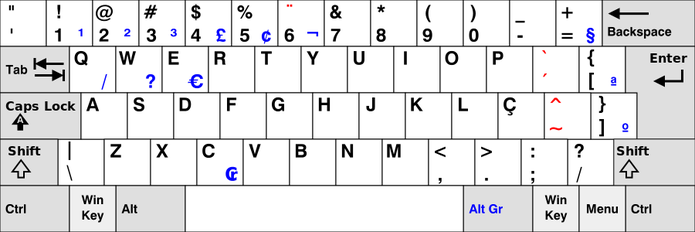
\includegraphics[width=1\linewidth]{Figuras/Ch02/fig19.1}
\end{frame}


\begin{frame}{Teclados no mundo}
	\begin{block}{}
		\begin{itemize}
			\item Cada local adota uma variante do teclado: na França usam o padrão AZERTY, e na Alemanha, o QWERTZ, por exemplo.
		\end{itemize}
	\end{block}

	\centering
	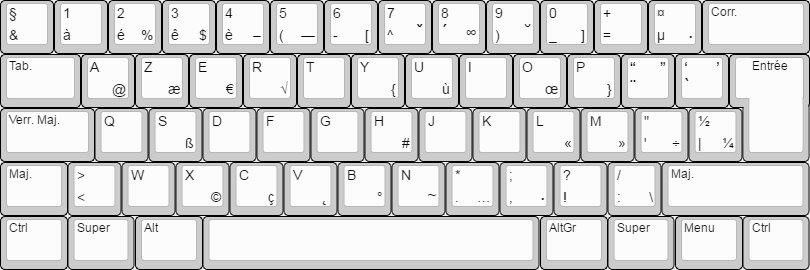
\includegraphics[width=0.7\linewidth]{Figuras/Ch02/fig19}

	\medskip

	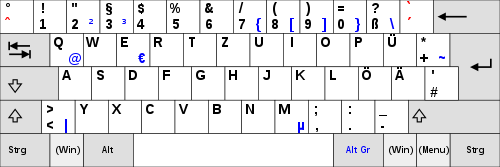
\includegraphics[width=0.7\linewidth]{Figuras/Ch02/fig20}

\end{frame}


\begin{frame}{Teclados no mundo}
	\begin{block}{}
		\begin{itemize}
			\item Teclado JCUKEN (para russo) e padrão japonês.
		\end{itemize}
	\end{block}

	\centering
	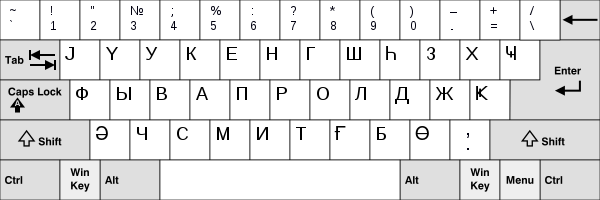
\includegraphics[width=0.75\linewidth]{Figuras/Ch02/fig24}

	\smallskip

	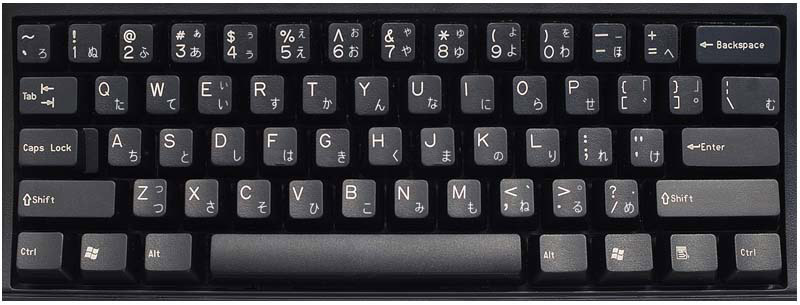
\includegraphics[width=0.75\linewidth]{Figuras/Ch02/fig25}
\end{frame}


\begin{frame}{Origem dos padrões}
	\begin{block}{}
		\begin{itemize}
			\item Esses padrões de teclado tem origem na época em que se usavam \textbf{máquinas de escrever}, e como ela possuía \textbf{peças mecânicas}, as teclas que eram usadas em conjunto deveriam ficar \textbf{mais longe} umas das outras, para que não houvesse problema na digitação rápida.
		\end{itemize}
	\end{block}

	\centering
	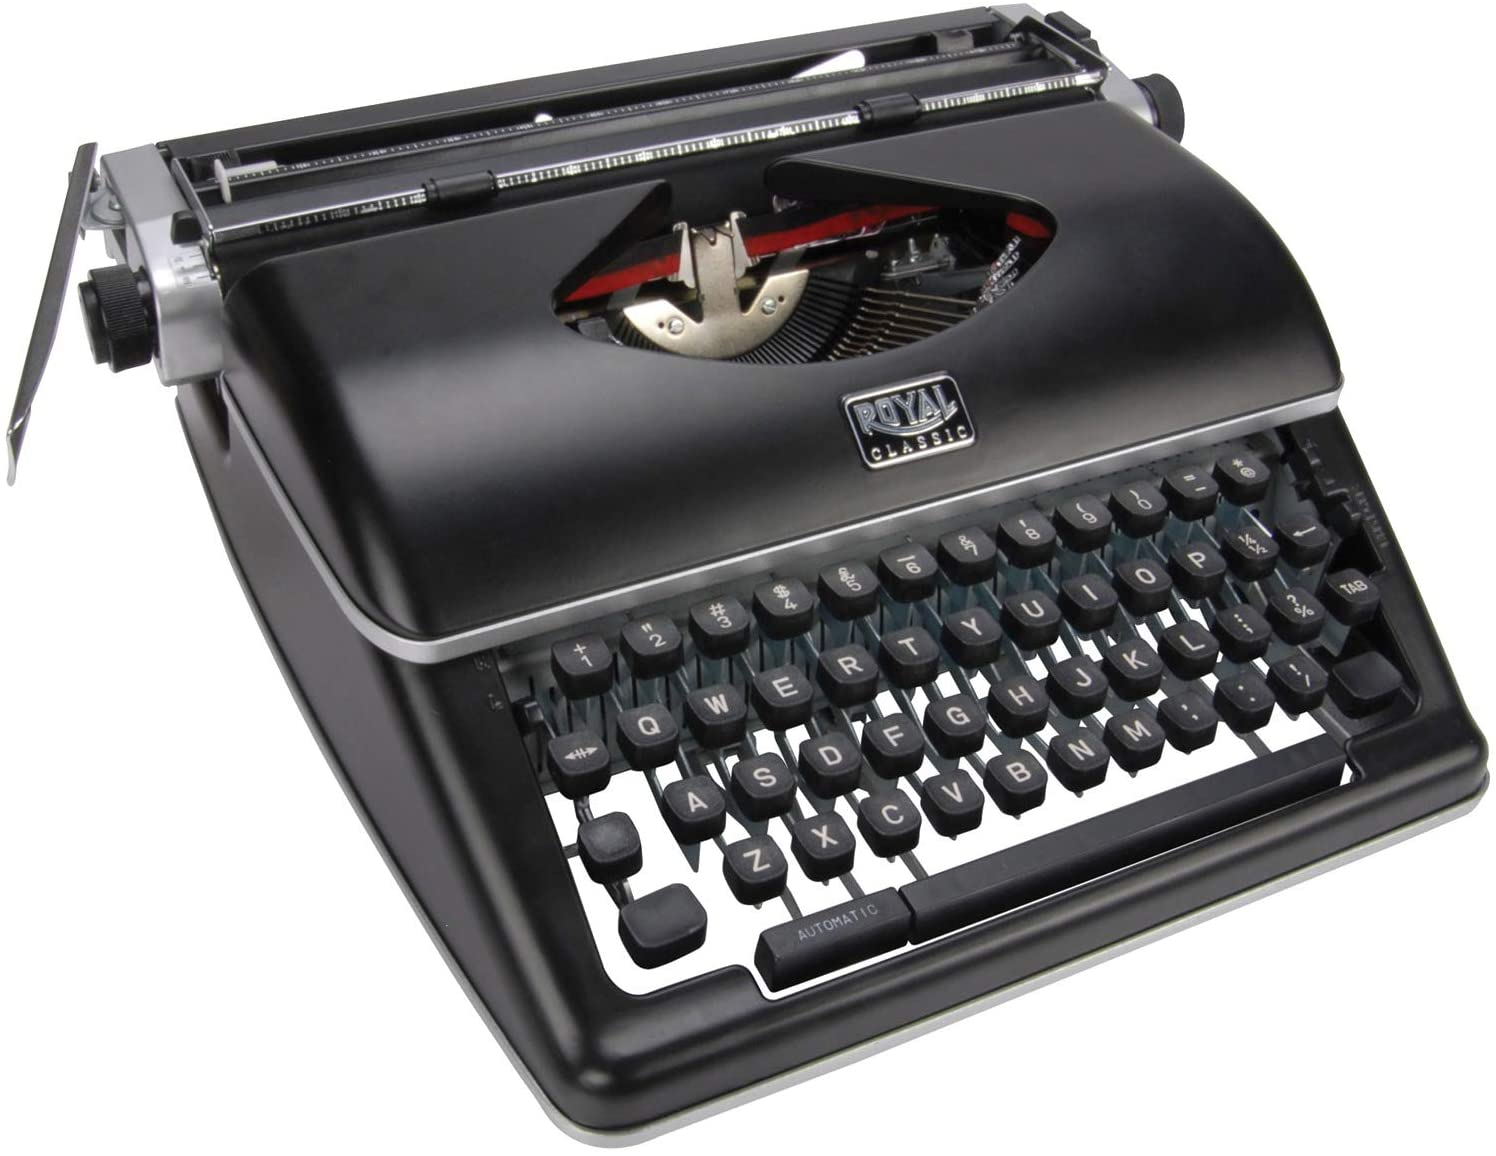
\includegraphics[width=0.6\linewidth]{Figuras/Ch02/fig19.2}
\end{frame}


\begin{frame}{Importância da Informação}
	\begin{block}{Malwares}
		\begin{itemize}
			\item Se o se computador “morresse” ou fosse infectado hoje, o que você perderia?
			      \begin{itemize}
				      \item\normalsize Fotos e vídeos de sua família?
				      \item\normalsize Trabalhos escolares?
				      \item\normalsize Documentos de trabalho?
			      \end{itemize}
			\item E se o computador com problemas fosse...
			      \begin{itemize}
				      \item\normalsize De uma empresa?
				      \item\normalsize De uma repartição pública?
				      \item\normalsize De uma base militar?
			      \end{itemize}
			\item Os \textit{malwares} são as \textbf{pragas virtuais}, que tem por foco causar algum tipo de \textbf{dano} ao \textbf{computador} ou ao \textbf{seus dados}.
		\end{itemize}
	\end{block}
\end{frame}


\begin{frame}{Ameaças virtuais}
	\begin{block}{Adware}
		\begin{itemize}
			\item \textit{ad} $ = $ anúncio, \textit{ware} vem de \textit{software}.
			\item Executa automaticamente e exibe uma grande quantidade de anúncios sem a \textbf{permissão} do usuário.
		\end{itemize}
	\end{block}

	\centering
	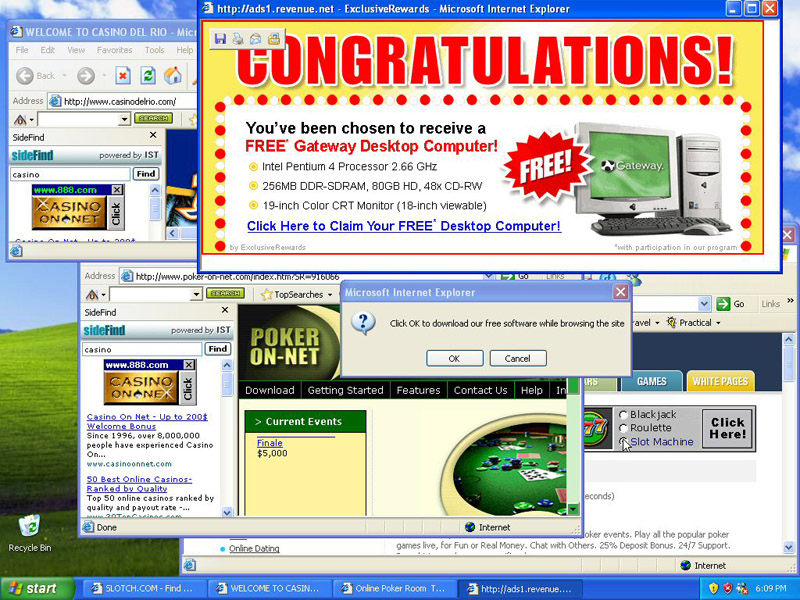
\includegraphics[width=0.6\linewidth]{Figuras/Ch02/fig26}
\end{frame}


\begin{frame}{Ameaças virtuais}
	\begin{block}{Browser hijacker}
		\begin{itemize}
			\item Sequestro de \textbf{navegador}.
			\item Altera as principais configurações do navegador (homepage, mecanismo de busca, etc) ou exibe anúncios em sites legítimos que redirecionam a vítima para sites maliciosos.
		\end{itemize}
	\end{block}

	%	\centering
	%	\includegraphics[width=0.7\linewidth]{Figuras/Ch02/fig}
\end{frame}


\begin{frame}{Ameaças virtuais}
	\begin{block}{Trojan (horse)}
		\begin{itemize}
			\item Cavalo de Troia
			\item Tem como objetivo manter-se \textbf{oculto} enquanto baixa e instala ameaças mais robustas nos computadores.
		\end{itemize}
	\end{block}

	\begin{block}{Rogueware}
		\begin{itemize}
			\item É um vampiro que busca sugar suas \textbf{informações confidenciais} para roubar dinheiro.
			\item Passam-se por programas de segurança e de otimização, e são abertos sem a interferência do usuário, exibindo resultados de uma varredura por vírus, que mostram a detecção de diversas “infecções”.
		\end{itemize}
	\end{block}
\end{frame}


\begin{frame}{Ameaças virtuais}
	\begin{block}{Spyware}
		\begin{itemize}
			\item Programa \textbf{espião} utilizado para captar informações sobre costumes dos usuários na internet, com o propósito de distribuir propaganda “customizada”.
		\end{itemize}
	\end{block}

	\begin{block}{Worm (verme)}
		\begin{itemize}
			\item Pode se auto-replicar sem a necessidade de infectar arquivos legítimos, criando \textbf{cópias funcionais} de si mesmos. Essas características permitem que os \textit{worms} se espalhem por redes de computadores e drivers USB.
		\end{itemize}
	\end{block}
\end{frame}


\begin{frame}{Ameaças virtuais}
	\begin{block}{Keylogger}
		\begin{itemize}
			\item Monitora, armazena e envia todas as \textbf{teclas} digitadas pela vítima.
			\item Atualmente, os keyloggers são incorporados em outros códigos maliciosos como trojans, para o roubo de logins ou dados bancários.
		\end{itemize}
	\end{block}

	\begin{block}{Ransomware}
		\begin{itemize}
			\item Sequestra arquivos ou todo o sistema da vítima por meio de técnica de \textbf{criptografia}.
			\item Após o “sequestro”, o malware exibe mensagens exigindo dinheiro ou compra de produtos para liberação dos arquivos.
		\end{itemize}
	\end{block}
\end{frame}


\begin{frame}{Cuidados com a segurança}
	\begin{block}{Formas de contaminação}
		Falha de segurança do sistema operacional ou navegador
		\begin{itemize}
			\item \textbf{Prevenção:} atualização constante dos sistemas e softwares.
		\end{itemize}
		Falha de segurança na rede
		\begin{itemize}
			\item \textbf{Prevenção:} atualização constante dos sistemas.
		\end{itemize}
		Uso de software infectado
		\begin{itemize}
			\item \textbf{Prevenção:} verificação com antivírus e instalação somente de softwares de fontes confiáveis.
		\end{itemize}
	\end{block}
\end{frame}


\begin{frame}{Cuidados com a segurança}
	\begin{block}{E-mail}
		\begin{itemize}
			\item Não clique em \textbf{links desconhecidos} ou \textbf{não solicitados}.
			\item Se você precisa acessar um endereço eletrônico, dê preferência em digitá-lo no navegador em vez de clicar em \textbf{links suspeitos}.
			\item Não confie em \textit{e-mails} cujo remetente é \textbf{desconhecido}.
			\item Cuidado com os \textit{spams}.
			\item Não baixe arquivos recebidos que desconheça ou não tenha solicitado.
			\item Após baixar um arquivo, verifique-o com um antivírus (mesmo que você conheça o remetente).
		\end{itemize}
	\end{block}
\end{frame}


\begin{frame}{Cuidados com a segurança}
	\begin{block}{Pendrive}
		\begin{itemize}
			\item Não use a opção “autoplay”.
			\item Escaneie os arquivos que quer utilizar (ou mesmo todo o pendrive) com um antivírus.
			\item Cuidado triplicado com pendrive de terceiros.
		\end{itemize}
	\end{block}
\end{frame}


\begin{frame}{Cuidados com a segurança}
	\begin{block}{Websites}
		\begin{itemize}
			\item Cuidado com o acesso a websites pouco confiáveis.
			\item Não instale “plugins requeridos” pelo website.
			\item Ao baixar arquivos, verifique se a extensão do arquivo corresponde ao que você esperava.
			\item Jamais abra arquivos ou execute programas sem antes verificar com um antivírus.
		\end{itemize}
	\end{block}
\end{frame}


\begin{frame}{Cópia de segurança}
	\begin{block}{Backup}
		\begin{itemize}
			\item O objetivo da cópia de arquivos permite a restauração dos mesmos em caso de \textbf{perda} ou \textbf{corrompimento} dos arquivos.
			\item É possível realizar backup (cópia de segurança) de todo o sistema ou só dos arquivos pessoais que você desejar proteger.
		\end{itemize}
	\end{block}
\end{frame}


\begin{frame}{Cópia de segurança}
	\begin{block}{Backup}
		Algumas opções para realizar a cópia de segurança:
		\begin{itemize}
			\item Opção de cópia de segurança (presente no SO).
			\item Software específico para backup e restauração de arquivos.
			\item Usando software que mantenha cópia de arquivos em nuvem, como Dropbox ou o Google Drive.
			\item Copiando manualmente os arquivos desejados para uma outra mídia de armazenamento (pendrive, HD externo, etc).
		\end{itemize}
	\end{block}
\end{frame}


\section*{Exercícios}
\frame{
	\frametitle{Exercícios}
	\begin{block}{}
		01. Descreva o funcionamento de um computador com as suas próprias palavras.

		\medskip

		02. Como você faria seu próprio vírus? O que ele faria com o computador ``hospedeiro''?
	\end{block}
}

\section*{Referências}

\frame{
	\frametitle{Referências e Exercícios Complementares}
	\begin{itemize}
		\item Gammack, John G.; Hobbs, Valerie; Pigott, Diarmuid (2011). The Book of Informatics (em inglês) revisada ed. [S.l.]: Cengage Learning.
	\end{itemize}
	%\centering{\alert{Página 36 - \textbf{1.6.1 até 1.6.5, 1.6.17 até 1.6.19}}} \\
	%	\centering{\alert{Lista de exercícios 01}}
}